\subsection{Using the same master check for both seed selectors}
The preceding distance control enters symbolic elimination directly,
while the learned method first checks the selected master basis.
To compare seed choices under the same admission procedure, we fixed
a second confirmation in which both selected sets receive the same
early check and full-pool fallback. The learned scores, threshold,
distance rule, twelve family instances and target batches stay
unchanged. The full-pool Kira control again uses its standard
supplied-equation reduction. We retained every measurement in the
first comparison.

Each method again uses five rotated repetitions on the same node
within a family and batch. This new comparison contains independent
timing repetitions of the same physical cases, so it checks the effect
of matching the admission procedure and does not introduce new
integral families. Complete times and descriptive intervals follow
the definitions in the preceding subsection.


The comparison with the same early check contains 360 records, of which 348 are measured trials. It produced 345 exact completions, 3 incomplete measured trials and 12 skipped repetitions. Independent checks evaluated 8,460 target coefficients against the raw Kira exports. All completed reductions matched their exact reference coefficients.

The learned method completed 115 trials exactly, with 1 failed trial and 4 skipped repetitions. Its completed trials required fallback 25 times.

The full-pool control completed 115 trials exactly, with 1 failed trial and 4 skipped repetitions. Its completed trials required fallback 0 times.

The distance control with the early check completed 115 trials exactly, with 1 failed trial and 4 skipped repetitions. Its completed trials required fallback 55 times.

Across both batch sizes, the learned complete-time ratio to the full-pool control is 0.932, with descriptive interval $[0.845,1.031]$ across 23 paired batches. The control completed 0 additional batches, while the learned method completed 0 additional batches.

For batches of 1 target, the learned complete-time ratio to the full-pool control is 0.914, with descriptive interval $[0.871,0.958]$ across 12 paired batches. The control completed 0 additional batches, while the learned method completed 0 additional batches.

For batches of 16 targets, the learned complete-time ratio to the full-pool control is 0.952, with descriptive interval $[0.772,1.148]$ across 11 paired batches. The control completed 0 additional batches, while the learned method completed 0 additional batches.

Across both batch sizes, the learned complete-time ratio to the distance control with the same early check is 0.925, with descriptive interval $[0.848,1.024]$ across 23 paired batches. The control completed 0 additional batches, while the learned method completed 0 additional batches.

For batches of 1 target, the learned complete-time ratio to the distance control with the same early check is 0.913, with descriptive interval $[0.855,0.972]$ across 12 paired batches. The control completed 0 additional batches, while the learned method completed 0 additional batches.

For batches of 16 targets, the learned complete-time ratio to the distance control with the same early check is 0.939, with descriptive interval $[0.764,1.136]$ across 11 paired batches. The control completed 0 additional batches, while the learned method completed 0 additional batches.

For the predefined single-target comparison, the learned method reduced geometric mean complete time by 8.6\% relative to the full pool and by 8.7\% relative to the distance rule with the same early check. Both descriptive intervals lie below one, and every method completed all five repeats for all twelve instances. The first confirmation gave a 7.8\% reduction relative to the full pool for this batch size. These results support a repeated gain for one constructed target expression at a time in this stored-identity setting. The sixteen-target intervals include one, so that batch size does not establish a consistent gain. The geometric means of the twelve per-family median complete times were 5.478 seconds for the full pool and 5.005 seconds for the learned method.

The learned workflow has an observed 6.8\% lower geometric mean complete time than the full-pool Kira control on batches where both methods completed all five repetitions. Because the descriptive interval includes one, the aggregate timing gain across both batch sizes remains uncertain. These conclusions concern reduction from the supplied identity pools and the tested constructed target expressions. Native equation generation, arbitrary scattering amplitudes and larger independent multiloop families remain outside this result \cite{KiraNativeAccelerationData}.

\begin{figure}[htbp]
\centering
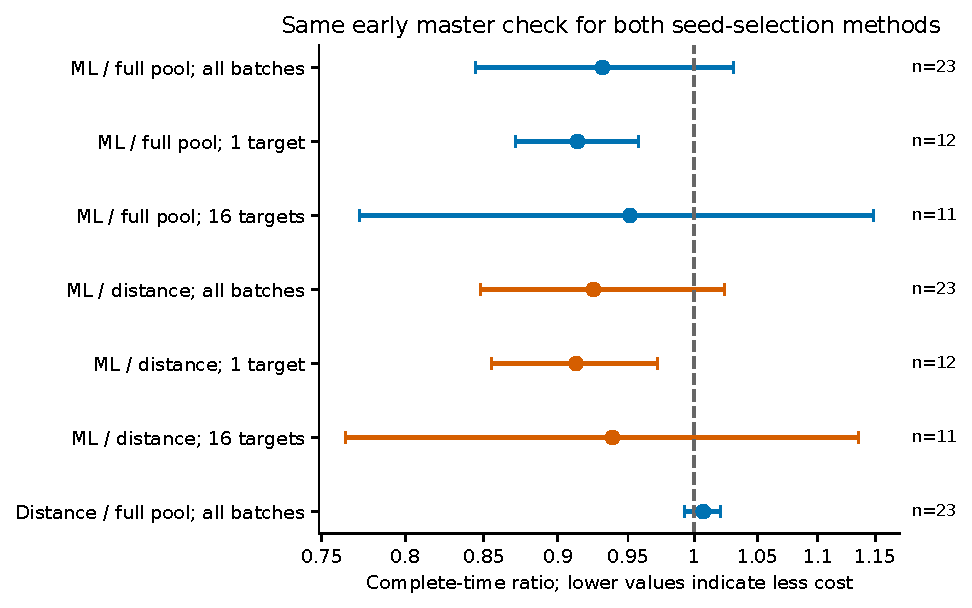
\includegraphics[width=\linewidth]{figures/whole_expression_matched_times.pdf}
\caption{Complete-time ratios with the same early master check for
learned and distance-selected seeds. Points show geometric means
of five-repeat median ratios, intervals resample kinematic groups,
and $n$ gives the number of complete paired batches. The full-pool
control uses standard supplied-equation Kira reduction.}
\label{fig:whole-expression-matched}
\end{figure}
\FloatBarrier

